\section[تمرین اول - سؤال دوم: خوشه‌بندی با DBSCAN]
{\faProjectDiagram\ \ تمرین اول ـ سؤال دوم: خوشه‌بندی داده‌ها با الگوریتم DBSCAN}

\begin{stepbox}

\field{هدف و معرفی مسئله}{
هدف این بخش، پیاده‌سازی الگوریتم خوشه‌بندی مبتنی بر چگالی (\lr{DBSCAN}) و بررسی عملکرد آن روی یک مجموعه داده دوبعدی بود. برخلاف الگوریتم K-Means که تعداد خوشه‌ها باید از قبل مشخص شود، الگوریتم DBSCAN با استفاده از چگالی نقاط، خوشه‌ها را به صورت خودکار شناسایی کرده و همچنین قادر به تشخیص نقاط نویز نیز می‌باشد.

مجموعه داده مورد استفاده شامل 4406 نمونه و دو ویژگی عددی بود که خروجی الگوریتم \lr{t-SNE} را نمایش می‌دهد و برای انجام خوشه‌بندی مناسب است.
}

\field{تعیین پارامترهای الگوریتم}{
الگوریتم DBSCAN به دو پارامتر اصلی نیاز دارد:

\begin{itemize}
\item $\varepsilon$ : شعاع همسایگی هر نقطه
\item \lr{MinPts} : حداقل تعداد نقاط لازم برای تشکیل یک ناحیه چگال
\end{itemize}

مطابق پیشنهاد رایج برای داده‌های دوبعدی، مقدار

\[
\text{MinPts}=2\times d = 4
\]

در نظر گرفته شد که در آن $d$ تعداد ابعاد داده است.

برای تعیین مقدار مناسب $\varepsilon$ ابتدا فاصله چهارمین همسایه نزدیک هر نمونه با استفاده از الگوریتم \lr{KNN} محاسبه شد. سپس با رسم نمودار فاصله‌ها و استفاده از الگوریتم \lr{KneeLocator}، نقطه زانویی منحنی استخراج و مقدار متناظر آن به عنوان مقدار مناسب $\varepsilon$ انتخاب گردید.

\vspace{0.4cm}

\begin{center}
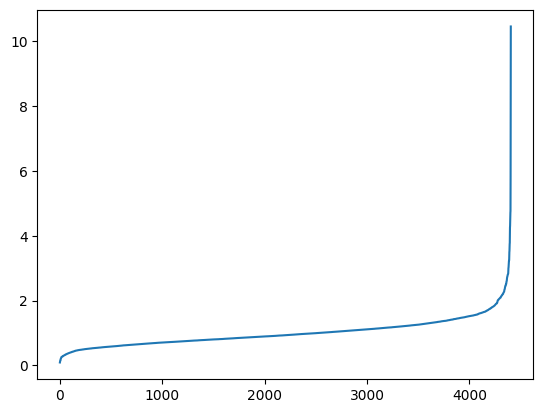
\includegraphics[width=.68\textwidth]{images/k_distance_plot.png}
\captionof{figure}{نمودار فاصله چهارمین همسایه و تعیین مقدار مناسب $\varepsilon$}
\label{fig:kdistance}
\end{center}
}


\field{اجرای الگوریتم DBSCAN}{
پس از تعیین پارامترهای الگوریتم، مدل DBSCAN با استفاده از کتابخانه \lr{Scikit-Learn} روی مجموعه داده اجرا شد. در پایان، هر نمونه به یکی از خوشه‌ها اختصاص داده شد و نقاطی که در هیچ ناحیه چگالی قرار نگرفتند، به عنوان نویز (\lr{Noise}) با برچسب $-1$ مشخص شدند.

\vspace{0.4cm}

\begin{center}
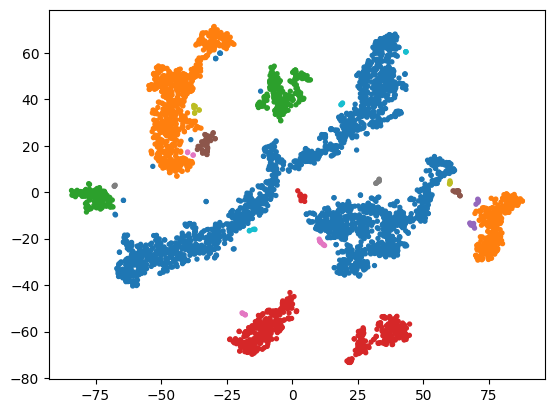
\includegraphics[width=.72\textwidth]{images/dbscan_clusters.png}
\captionof{figure}{نتیجه خوشه‌بندی داده‌ها توسط الگوریتم DBSCAN}
\label{fig:dbscan_result}
\end{center}
}


\field{نتایج و تحلیل}{
نتایج اجرای الگوریتم نشان داد که DBSCAN موفق به شناسایی

\[
\boxed{23}
\]

خوشه مختلف در مجموعه داده شده است. همچنین تعداد

\[
\boxed{34}
\]

نمونه به عنوان نقاط نویز شناسایی شدند که در هیچ ناحیه با چگالی کافی قرار نداشتند.

مزیت اصلی این الگوریتم نسبت به روش‌هایی مانند K-Means، عدم نیاز به تعیین تعداد خوشه‌ها و همچنین توانایی تشخیص نقاط پرت است. این ویژگی باعث می‌شود DBSCAN برای داده‌هایی با شکل‌های پیچیده و نامنظم عملکرد بسیار مناسبی داشته باشد.
}

\field{جمع‌بندی}{
در این تمرین الگوریتم DBSCAN با تعیین خودکار مقدار $\varepsilon$ به کمک نمودار فاصله همسایه‌ها و الگوریتم \lr{KneeLocator} پیاده‌سازی شد. نتایج نشان داد که این روش قادر است بدون اطلاع قبلی از تعداد خوشه‌ها، ساختار طبیعی داده‌ها را استخراج کرده و نقاط نویز را نیز به خوبی شناسایی نماید. به همین دلیل DBSCAN یکی از مناسب‌ترین روش‌های خوشه‌بندی برای داده‌های با توزیع نامنظم و دارای نقاط پرت محسوب می‌شود.
}

\end{stepbox}